\newpage
\subsection{Software Work}

% Give a brief software overview
\textbf{Software Brief: }
RIMA1 and RIMA2 ran off the ROS1 Melodic framework. They utilised custom messages and customised ROS packages to function. All code for the robot was written in C++ and analysis scripts used for PEC are written
in Python. Unfortunately the codebases for these robots cannot be shared as it is property of UTS and Sydney Water. The robots processes and GUI's are all run/launched ushing shell scripts in the linux CL.

% New RIMA1 system board software update
\vspace{\baselineskip}
\textbf{RIMA1 System Board Software Update: }
The new system board required some minor software updates. This primarily consisted of changes to message data types and names. This change also required small modification to RIMA1's core.cpp file which was resposible 
for ROS handling (i.e. setting up subscribers, publishers, etc.). 

% RIMA1 GUI Update
\vspace{\baselineskip}
\textbf{RIMA1 GUI Update: }
The old GUI of RIMA was outdated and not greatly designed and doing something simple such as turning required going into settings and modifying rotation setpoints which is clearly not ideal or user friendly. I updated
the GUI [~\ref{fig:r1gui}] to have more intuitive control, I also installed rear cameras at the time for rear view and visual view of the sensor to have a better cue of full expansion rather than basing it off the current reading. Basic 
IMU visualisation was also added to the GUI to allow for better understanding of the robot's orientation in the pipe. The GUI was written in C++ using Qt Designer.

\begin{figure*}[htbp]
    \centering
    \subfloat[Old RIMA1 interface]{
        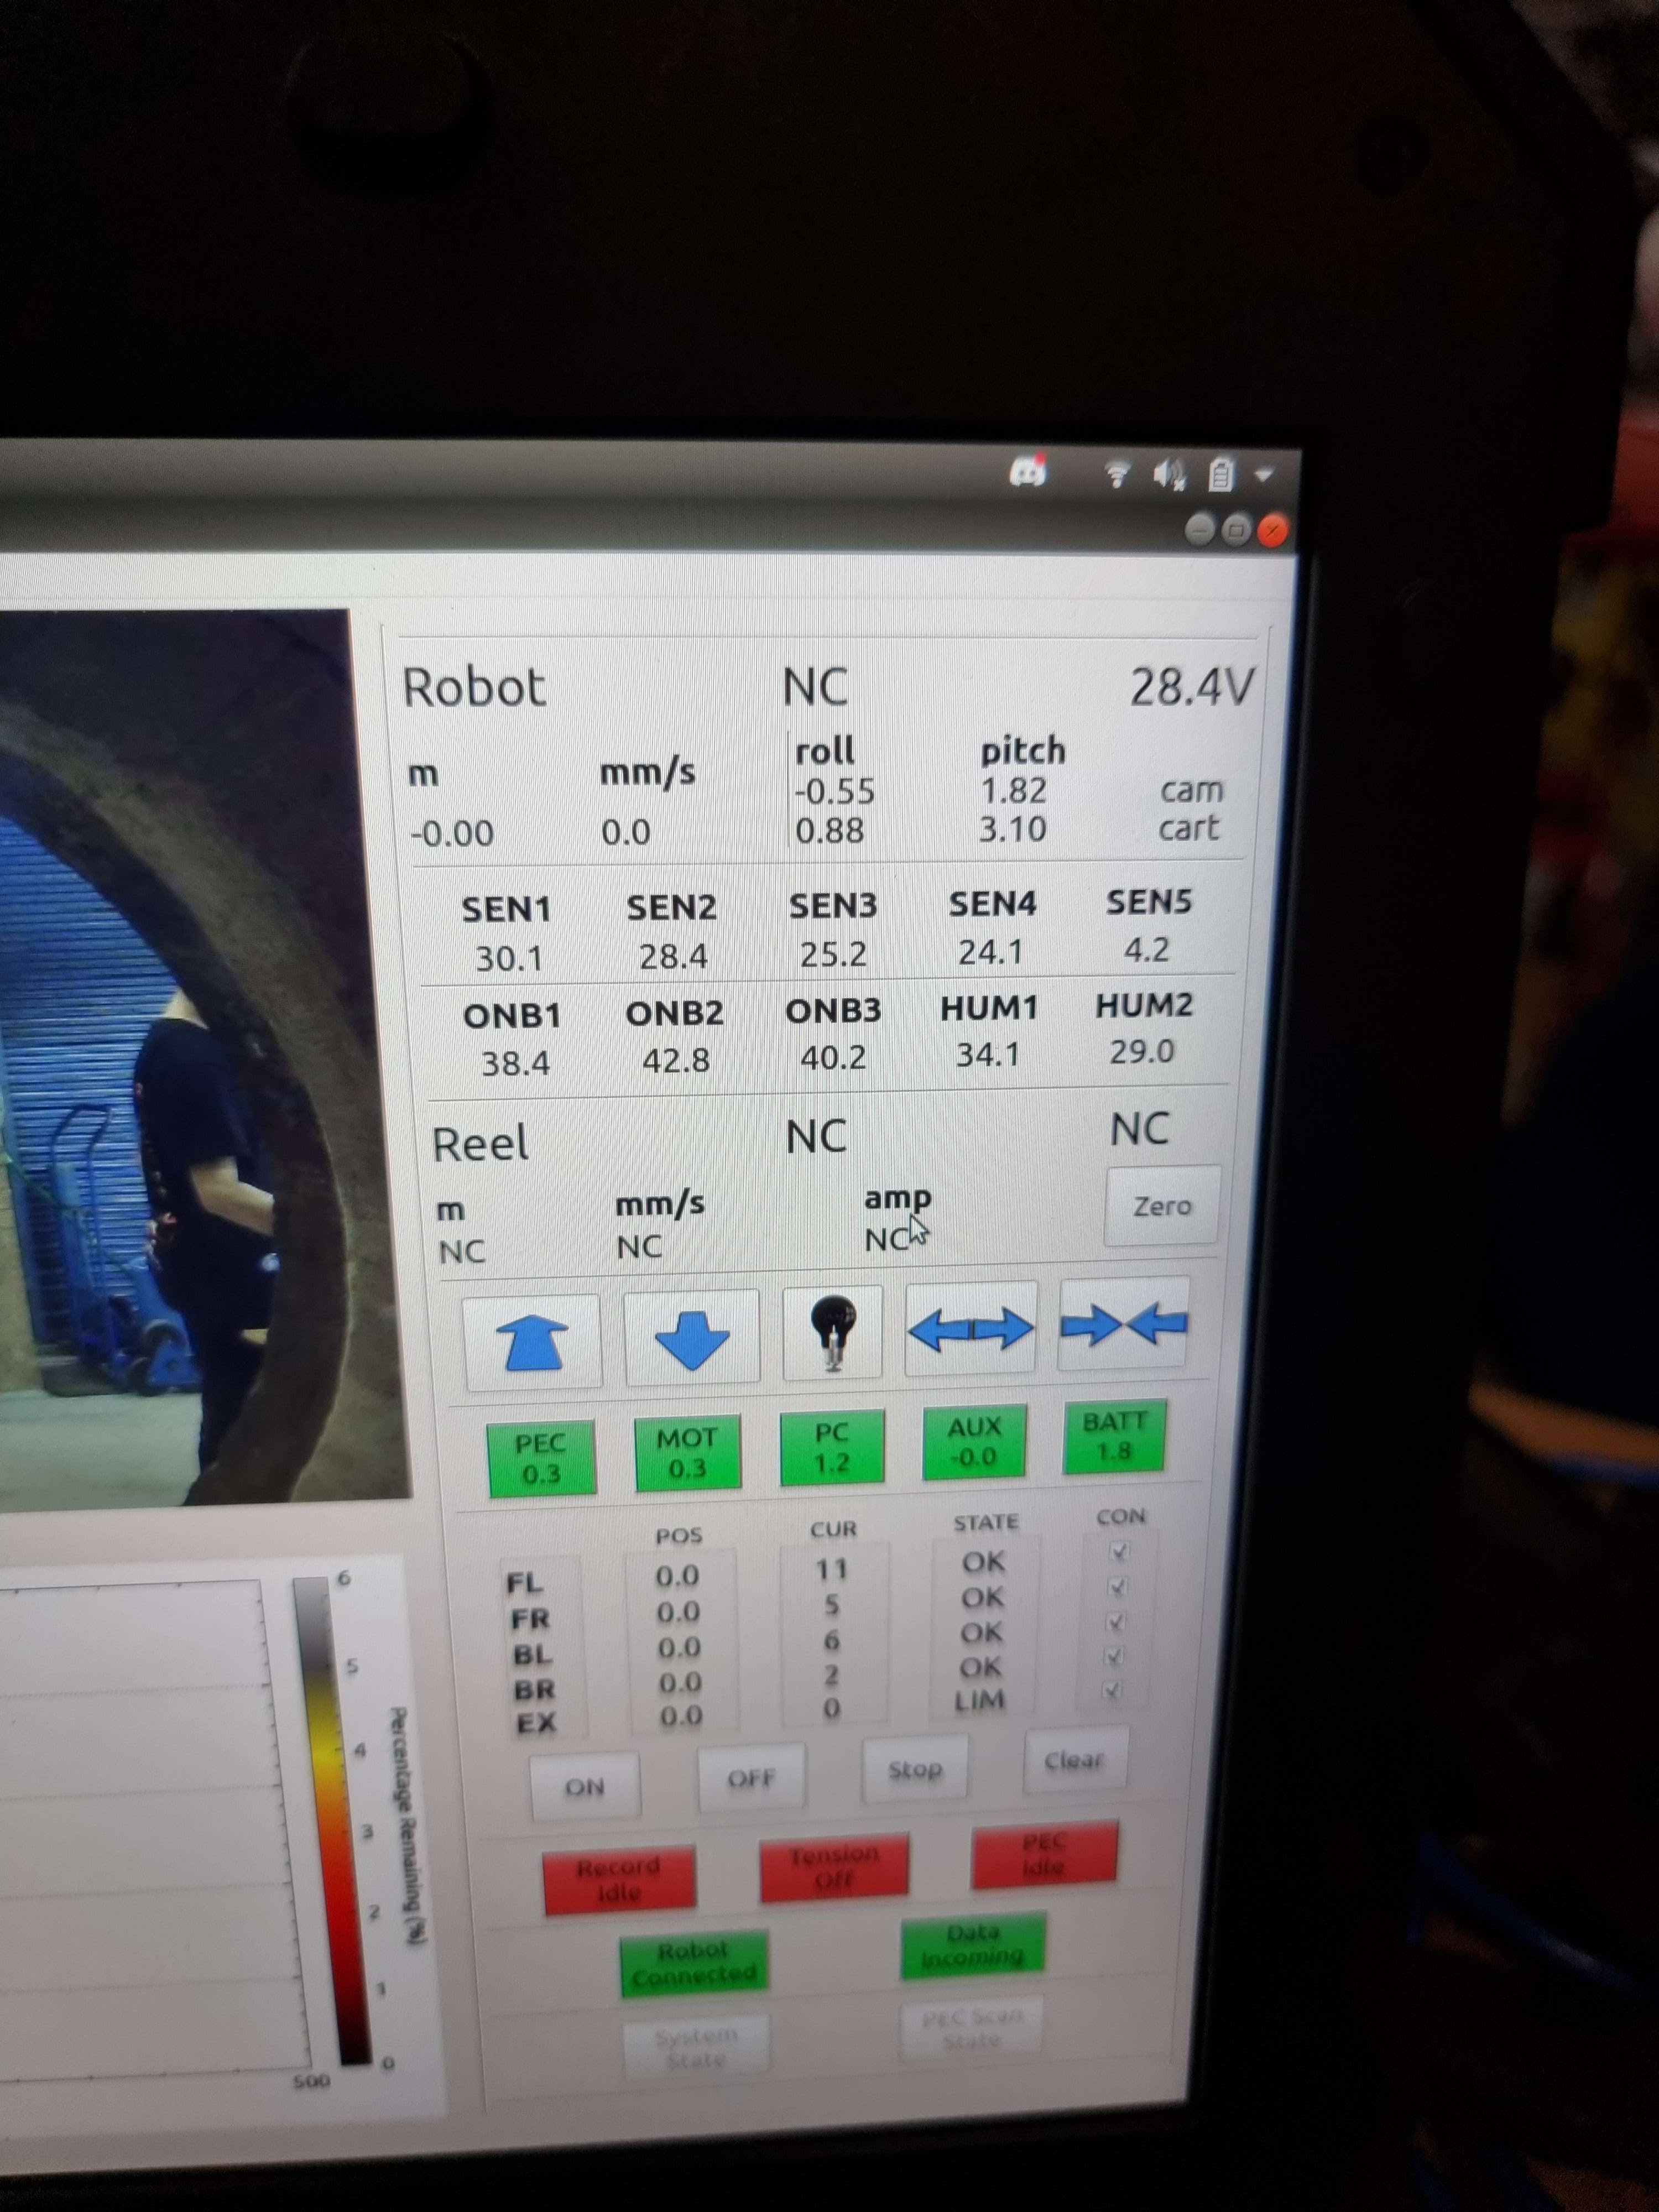
\includegraphics[width=0.30\textwidth, valign=c]{images/rima1/rima1_old_gui.jpg}
    }
    \hspace{0.5cm}
    \subfloat[New RIMA1 interface]{
        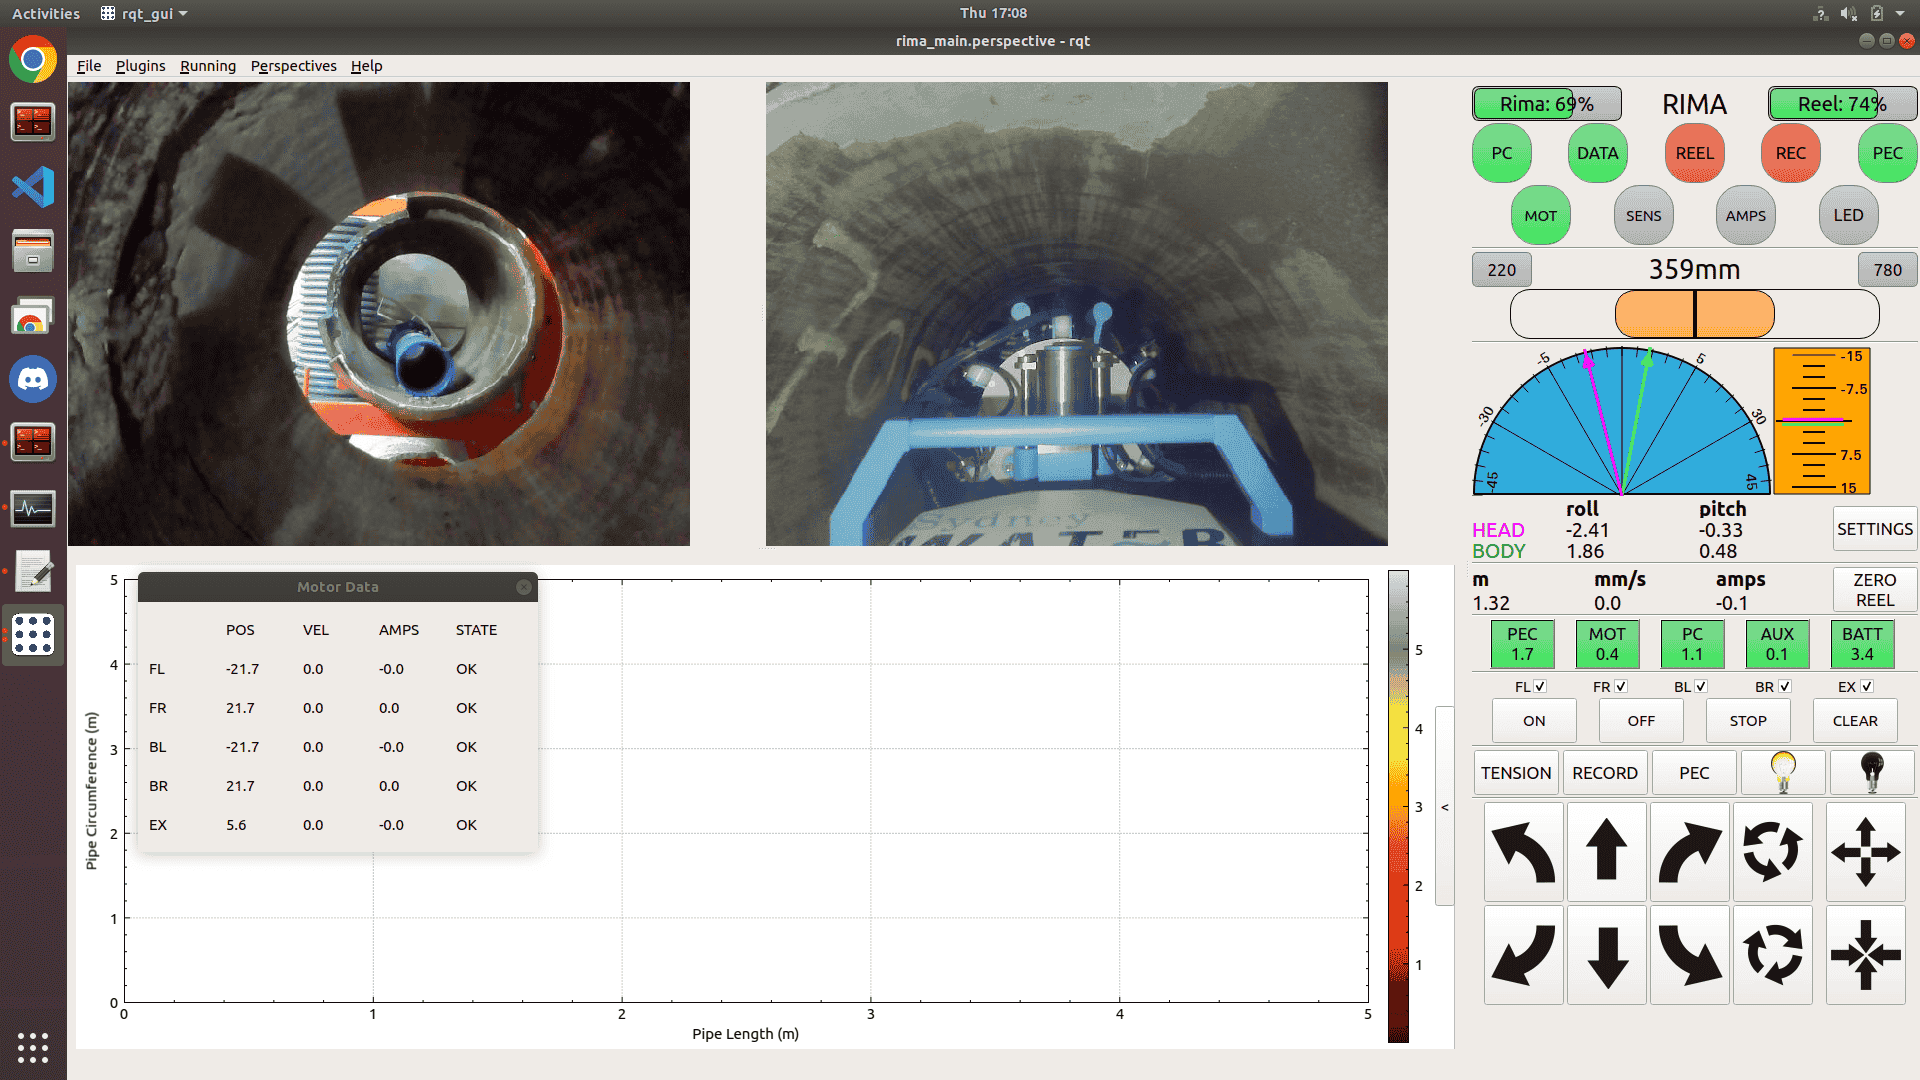
\includegraphics[width=0.60\textwidth, valign=c]{images/rima1/rima_gui_new.png}
    }
    \caption{Comparison of RIMA1 GUI's}
    \label{fig:r1gui}
\end{figure*}
\newpage
\imginin{rima1/rear_cam_rear.jpg}{RIMA1 Rear Camera rear View}{rcam}{0.8}

% Embedded software debugging for RIMA2 PEC

% PEC Calibration

% Simplified shell script for data tranfer
